%%%%%%%%%%%%%%%%%%%%%%%%%%%%%%%%%%%%%%%%%%%%%%%%%%%%%%%%%%%%%%%%%%%%%%%%%%%%%%%%
%2345678901234567890123456789012345678901234567890123456789012345678901234567890
%        1         2         3         4         5         6         7         8
\newcount\Comments  % 0 suppresses notes to selves in text
\Comments=1   % TODO: set to 0 for final version

% \documentclass[letterpaper, 10 pt, journal, twoside]{IEEEtran}	 % Comment this line out if you need a4paper

% %\documentclass[letterpaper, 10 pt, conference]{ieeeconf}  % Comment this line out if you need a4paper

% %\documentclass[a4paper, 10pt, conference]{ieeeconf}      % Use this line for a4 paper

% \IEEEoverridecommandlockouts                              % This command is only needed if 
%                                                           % you want to use the \thanks command

% \overrideIEEEmargins                                      % Needed to meet printer requirements.



\documentclass[letterpaper, 10 pt, conference]{ieeeconf}  % Comment this line out if you need a4paper

%\documentclass[a4paper, 10pt, conference]{ieeeconf}      % Use this line for a4 paper

\IEEEoverridecommandlockouts                              % This command is only needed if 
                                                          % you want to use the \thanks command

\overrideIEEEmargins                                      % Needed to meet printer requirements.



% See the \addtolength command later in the file to balance the column lengths
% on the last page of the document

% The following packages can be found on http:\\www.ctan.org
\usepackage{graphicx} % for pdf, bitmapped graphics files
\usepackage{epsfig} % for postscript graphics files
% \usepackage[T1]{fontenc}
% \usepackage{lmodern}
% \usepackage{mathtools, nccmath, textcomp} 
\usepackage{amsmath}
\usepackage{amsfonts}
\usepackage{amssymb}
\usepackage{multirow}
% \ifCLASSOPTIONcompsoc
%     \usepackage[caption=false, font=normalsize, labelfont=sf, textfont=sf]{subfig}
% \else
\usepackage[caption=false, font=footnotesize]{subfig}

\usepackage{algorithm,algpseudocode}
\renewcommand{\algorithmicrequire}{\textbf{Input:}}
\renewcommand{\algorithmicensure}{\textbf{Output:}}

% % for comments
% \usepackage[textwidth=1.9cm]{todonotes}
% \setlength{\marginparwidth}{1.5cm}
% \newcommand{\igor}[2][] {\todo[color=red, #1]		{IGOR: #2}}
% \newcommand{\simeon}[2][] {\todo[color=cyan, #1]		{SIMEON: #2}}
% % \newcommand{\ryu}[2][]  {\todo[color=green, #1]		{RYU: #2}}
% % \newcommand{\JH}[1]{\color{red} {\bf (JH: #1)}} 


\DeclareMathOperator{\E}{\mathbb{E}}
\DeclareMathOperator*{\argmin}{argmin}
\DeclareMathOperator*{\argmax}{argmax}

%\title{\LARGE \bf Dynamic Model of Twisted String Actuators that Accounts for Friction and Elastic Deformations}
%\title{\LARGE \bf Accurate Torque Modeling of Twisted String Actuators by Accounting for String Compliance and Friction}

\markboth{IEEE Robotics and Automation Letters. Preprint Version. Accepted January, 2020}{Nedelchev \MakeLowercase{\textit{et al.}}: Dynamic Modeling of Twisted String Actuators} 
% Use only for final RAL version


\title{On Energy-Preserving Motion in Twisted String Actuators}

% \title{\LARGE \bf Parameter Identification in Dynamical Systems with Energy-Based Regressor: Preliminary Study }


 \author{Simeon Nedelchev$^1$, Valeria Skvortsova$^1$, Boris Guryev$^1$, Igor Gaponov$^1$,~Jee-Hwan Ryu$^2$ % <-this % stops a space
% 	\thanks{The research is supported by grant of the Russian Science Foundation project No:19-79-10246}% <-this % stops a space  
     \thanks{*The reported study was funded by RFBR and National Research Foundation of Korea according to the research project No. 19-58-51014.}
     \thanks{$^1$Institute of Robotics and Computer Vision, Innopolis University, Innopolis, Russia. {\tt\footnotesize  \{s.nedelchev, v.skvortsova\}@innopolis.university,  \{b.guryev, i.gaponov\}@innopolis.ru}.}
    \thanks{ $^2$Department of Civil and Environmental Engineering, KAIST, Daejeon, South Korea. \tt\footnotesize jhryu@kaist.ac.kr.}
 }

% \def\eref#1{(\ref{#1})}
\usepackage{array}
\newcolumntype{P}[1]{>{\centering\arraybackslash}p{#1}}

\begin{document}
	\maketitle 
	\thispagestyle{empty}
	\pagestyle{empty}
	%%%%%%%%%%%%%%%%%%%%%%%%%%%%%%%%%%%%%%%%%%%%%%%%%%%%%%%%%%%%%%%%%%%%%%%%%%%%%%%%
	\begin{abstract}
	Many applications require robotic end-effectors and mechanisms to move along periodic trajectories of given amplitude and frequency.
If motion parameters are known in advance, it might be beneficial to design the mechanism in such a way that its natural frequency is close to that of the desired trajectory so that controller needs to provide minimal effort to generate sustained oscillations. 
In this paper, we investigate natural nonlinear oscillatory behavior in twisted  string  actuators (TSA), describing its mathematical model and providing experimental verification of this phenomenon based on observations of dynamics and energy.
We also design an energy-preserving controller that is capable of generating undamped oscillations of desired magnitude even under severe constraints on actuator torque.
Experimental study has demonstrated that it was possible to induce undamped oscillatory response of TSA with a 2-kg payload while applying a maximum of 6 mNm motor torque, which can be used in robotic applications that require periodic motions and high controller efficiency, like legged robots.
	\end{abstract}	
	% 	Keywords: twisted string actuator, adaptive control, cable transmission. 
%	Keywords: a parameter identification, energy-based regressor, energy equations of motions
	%%%%%%%%%%%%%%%%%%%%%%%%%%%%%%%%%%%%%%%%%%%%%%%%%%%%%%%%%%%%%%%%%%%%%%%%%%%%%%%%
	
    %Various applications of mechanical engineering and robotics involve periodic motion of the end-effectors, links and payloads. These include legged robots, lower-limb exoskeletons, mechanisms providing cyclic motion, and many others. One of the key aspects in control over such systems is their energy efficiency. This calls for the use of lightweight actuators with high power density and efficient control schemes for them. 

Twisted string actuators (TSAs) are rotary-to-translational cable-driven actuators, in which torsional twisting of a bundle of strings or cables results in their contraction. Key advantages of TSAs include light weight, high efficiency and power density, and compliance. These actuators are used in various applications including multi-legged robots \cite{suzuki2005toward}, lower-limb exoskeletons \cite{kornbluh2018twisted} and mobile robots \cite{sabelhaus2015system}, all of which involve periodic motion of the payload. However, the dynamical properties of TSAs have not been fully explored in these studies, with the authors mainly employing the actuators for low-speed control. However, these applications involved comparatively low payload forces \cite{nedelchev2020accurate}. When operating with significant payload during high-frequency motion, a more efficient control approach might be required.

Conventionally, TSAs are controlled in a uni-directional fashion when the motor twists the strings from their initial state all the way until desired contraction level is reached, and then back. Thus, if a fast periodical motion of the payload is required, the motor needs to be stopped and reversed 4 times during each period, around both zero and fully twisted positions, which may cause power losses since the energy generated by motor driver should be sufficient to overcome the kinetic energy of spinning rotor inertia when stopping. However, one of the unique features of the TSAs is their symmetrical behaviour: the strings contract identically whether they are twisted clockwise or counterclockwise. With this in mind, one can design a control system in such a way that the motor twists the strings in both directions, which will eliminate the need to reverse the motor in its zero configuration. An additional benefit is that motor's shaft itself, despite its comparatively low inertia, can propel the payload by twisting the strings on its own without drawing any power from the supply. As a consequence, a TSA-driven system with proposed controller can reach higher string contraction values with constraints on motor torque.

%In this paper, we implement an energy-preserving control in application to twisted string actuators. 
We have observed during the experiments that when the loaded twisted strings were released freely from their contracted state, they  twisted in the opposite direction on their own after being completely untwisted, carried on by the motor inertia. As the result, the strings contracted again, sometimes working against significant forces that acted on the payload, with no effort required from the actuator. This held true even for comparatively small values of rotor inertia.
Thus, knowing some intrinsic properties of a TSA-powered setup such as its natural frequency, one can leverage the tendency of TSA to oscillate freely in order to design an efficient controller which will be able to induce periodical motion of the payload with minimal motor power required. This controller can maintain the mechanical energy of the system at a desired, constant level by compensating for the power losses within the system, effectively turning the setup into a frictionless nonlinear pendulum. In this work, we have implemented an energy-preserving control law on a practical linear TSA setup, and designed it so that it supported undamped oscillatory response of a 2-kg payload with desired magnitude and natural frequency while  requiring a maximum of 6 mNm torque from the actuator. 

To the best of our knowledge, this paper marks the first occasion when free oscillations in TSA systems were studied, modeled, and experimentally investigated. In addition, this work presents novel experimental results on the application of energy-preserving control to TSA-based robotic systems. Such systems and controllers can be used in the limbs of bipedal and quadruped robots to ensure energy-efficient locomotion, even in the presence of severe actuator limitations.



    \section{Introduction}
Various applications of mechanical engineering and robotics involve periodic motion of the end-effectors, links and payloads. These include legged robots, lower-limb exoskeletons, mechanisms providing cyclic motion, and many others. One of the key aspects in control over such systems is their energy efficiency. This calls for the use of lightweight actuators with high power density and efficient control schemes for them. 

Twisted string actuators (TSAs) are rotary-to-translational cable-driven actuators, in which torsional twisting of a bundle of strings or cables results in their contraction. Key advantages of TSAs include light weight, high efficiency and power density, and compliance. These actuators are used in various applications including multi-legged robots \cite{suzuki2005toward}, lower-limb exoskeletons \cite{kornbluh2018twisted} and mobile robots \cite{sabelhaus2015system}, all of which involve periodic motion of the payload. However, the dynamical properties of TSAs have not been fully explored in these studies, with the authors mainly employing the actuators for low-speed control. However, these applications involved comparatively low payload forces \cite{nedelchev2020accurate}. When operating with significant payload during high-frequency motion, a more efficient control approach might be required.

Conventionally, TSAs are controlled in a uni-directional fashion when the motor twists the strings from their initial state all the way until desired contraction level is reached, and then back. Thus, if a fast periodical motion of the payload is required, the motor needs to be stopped and reversed 4 times during each period, around both zero and fully twisted positions, which may cause power losses since the energy generated by motor driver should be sufficient to overcome the kinetic energy of spinning rotor inertia when stopping. However, one of the unique features of the TSAs is their symmetrical behaviour: the strings contract identically whether they are twisted clockwise or counterclockwise. With this in mind, one can design a control system in such a way that the motor twists the strings in both directions, which will eliminate the need to reverse the motor in its zero configuration. An additional benefit is that motor's shaft itself, despite its comparatively low inertia, can propel the payload by twisting the strings on its own without drawing any power from the supply. As a consequence, a TSA-driven system with proposed controller can reach higher string contraction values with constraints on motor torque.

%In this paper, we implement an energy-preserving control in application to twisted string actuators. 
We have observed during the experiments that when the loaded twisted strings were released freely from their contracted state, they  twisted in the opposite direction on their own after being completely untwisted, carried on by the motor inertia. As the result, the strings contracted again, sometimes working against significant forces that acted on the payload, with no effort required from the actuator. This held true even for comparatively small values of rotor inertia.
Thus, knowing some intrinsic properties of a TSA-powered setup such as its natural frequency, one can leverage the tendency of TSA to oscillate freely in order to design an efficient controller which will be able to induce periodical motion of the payload with minimal motor power required. This controller can maintain the mechanical energy of the system at a desired, constant level by compensating for the power losses within the system, effectively turning the setup into a frictionless nonlinear pendulum. In this work, we have implemented an energy-preserving control law on a practical linear TSA setup, and designed it so that it supported undamped oscillatory response of a 2-kg payload with desired magnitude and natural frequency while  requiring a maximum of 6 mNm torque from the actuator. 

To the best of our knowledge, this paper marks the first occasion when free oscillations in TSA systems were studied, modeled, and experimentally investigated. In addition, this work presents novel experimental results on the application of energy-preserving control to TSA-based robotic systems. Such systems and controllers can be used in the limbs of bipedal and quadruped robots to ensure energy-efficient locomotion, even in the presence of severe actuator limitations.




\section{Mathematical Modeling of TSA}
\label{modeling}
Before proceeding to the analysis of natural oscillations in twisted string actuators, we would like to start with a brief overview of the mathematical modeling of TSA. For a deeper insight and peculiarities of TSA modeling, the reader may refer to previously published works \cite{nedelchev2020accurate}, \cite{popov2012study}, \cite{palli2012modeling}.

\subsection{Kinematics}
% \subsubsection*{Mathematical Model of a TSA}




According to the conventional representation of a section of twisted string shown in Fig. \ref{fig:schematic_diagram}(a), a cable of length $L$ and radius $r$, twisted at an angle $\theta$, forms a helix and contracts by the $X$ amount. For the resulting right triangle with the sides $(L-X),\theta r$, and $L$ one can derive the geometric constraint of twisted string as:
\begin{equation}\label{eq.mod:geom_const}
\theta^2 r^2 + (L-X)^2 - L^2 = 0  
\end{equation}

It is important to note here that equation above is a second order polynomial, and there exist two solutions for motor angle $\theta$ that correspond to \textit{the same contraction level} $X$.

Differentiating the constraint above yields the relationships between the payload (output) and motor (input) velocities:
\begin{equation}\label{eq.mod:x_dot}
\dot{X} = \mathcal{J}(\theta, X)\dot{\theta}
\end{equation}
where $J$ denotes the Jacobian of twisted strings and $\dot{\theta}$ stands for angular speed. Hereinafter, we will omit the arguments $(\theta, X)$ for the sake of brevity.


It is worth noting that the twisted strings Jacobian may be represented in various ways, depending on the availability of motor or payload variables:
\begin{equation}\label{eq.mod:jacobian}
    \mathcal{J} = \frac{\theta r^2}{L-X} = \frac{\theta r^2}{\sqrt{L^2 - \theta^2 r^2}} = \frac{r \sqrt{L^2 - (L -X)^2}}{L-X} 
\end{equation}

\subsection{Energy}
Total energy of TSA can be represented just like that of any conventional mechanical system as a sum of kinetic, potential and dissipated energy terms $E = E_K + E_P + E_D$ as follows:
\begin{equation}\label{eq.mod:total_energy}
    E = \frac{1}{2} I\dot{\theta}^2 + \frac{1}{2}m \dot{X}^2 + mgX + E_D
\end{equation}
where the first term represents kinetic energy of the spinning motor shaft with inertia $I$, the next two terms correspond to kinetic energy of the payload of mass $m$ moving at speed $\dot{X}$ and its potential energy due to gravity (here we assume the payload always moves along the vertical axis), with $g$ denoting the gravitational constant, while the term $E_D$ represents all the energy losses due to friction inside the motor, payload's sliders and the strings themselves, as well as reflecting all other internal and external disruptive forces, otherwise unaccounted for explicitly.


\begin{figure}
		\centering
		\vspace*{2mm} 
		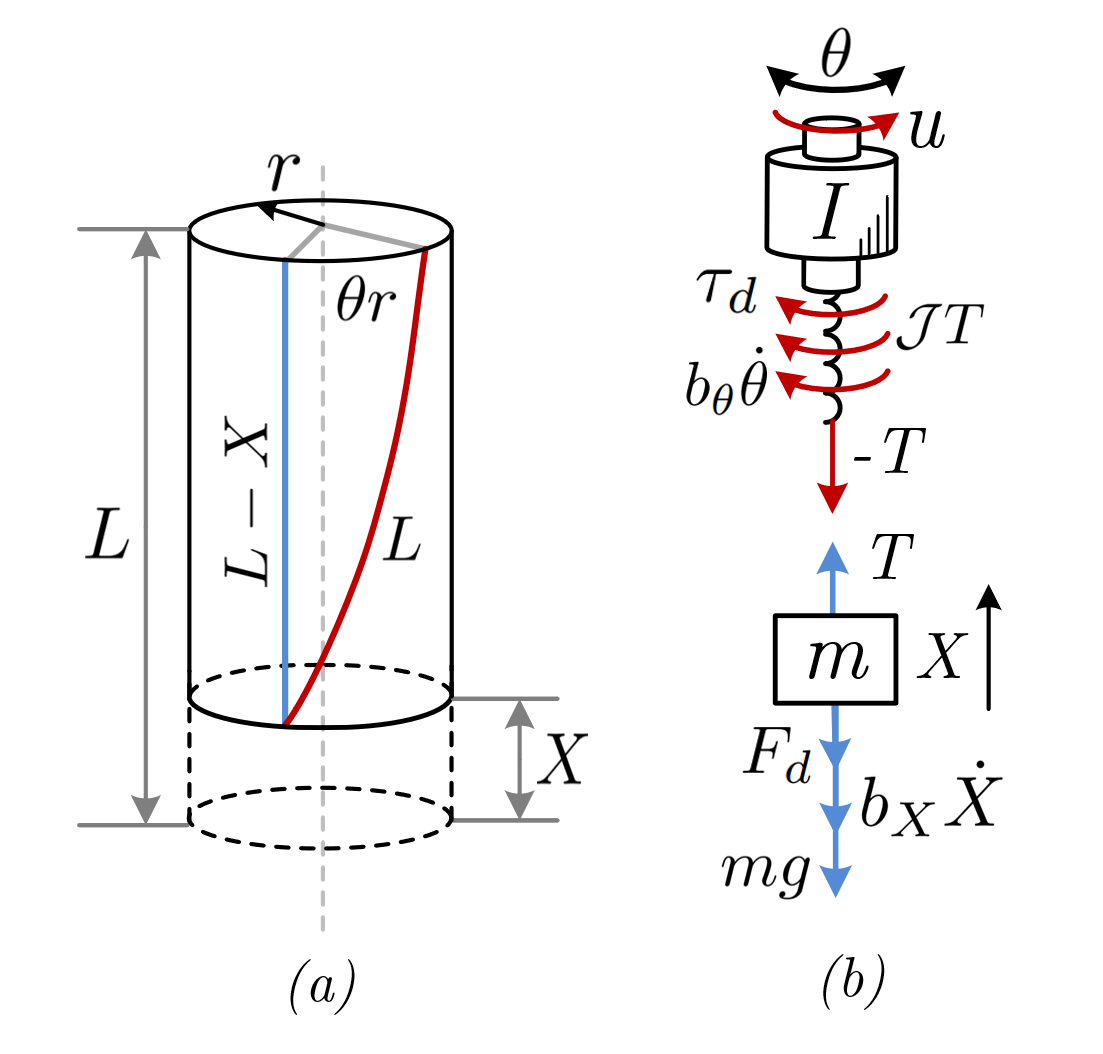
\includegraphics[trim= 0.0cm 1.0cm 0.0cm 0.0cm,width=0.72\columnwidth]{pics/tsa_scheme.PNG}
		\caption{Schematic diagrams for the analysis of TSA kinematics (a) and dynamics (b)}
		\label{fig:schematic_diagram}
\end{figure}
Depending on the variables of choice, one may represent the kinetic and potential energy with the motor-side or payload-side variables using the kinematical constraints \eqref{eq.mod:x_dot} and \eqref{eq.mod:jacobian} as follows:
\begin{equation}\label{eq.mod:K_Pi_energies}
\begin{matrix}
    E_K = \frac{1}{2} (I + m \mathcal{J}^2)\dot{\theta}^2 = \frac{1}{2} (I\mathcal{J}^{-2} + m )\dot{X}^2 \\ 
    \\
    E_P = mgX = mg (L - \sqrt{L^2 - \theta^2r^2} )  \\ 
\end{matrix}
\end{equation}
where terms preceding the squares of velocities $\dot{\theta}^2, \dot{X}^2$ represent the reflected inertia values on the motor and payload sides, respectively. 

\subsection{Dynamics}
A schematic diagram of a twisted string actuator with a connected payload is shown in Fig. \ref{fig:schematic_diagram} (b). After driving the energy equations, one may use Lagrange-Euler approach to derive the equations of motion (EoM) of twisted string actuators as follows:
\begin{equation}\label{eq.mod:dyn_model}
\left\{\begin{matrix}
u = I \ddot{\theta} + \mathcal{J}T  + b_\theta \dot{\theta} + \tau_{d}
\\[0.5em]
T = m \ddot{X} + mg  + b_X \dot{X} + F_{d}
\end{matrix}\right.
\end{equation}
where $u$ denotes motor torque, $T$ stands for string's tension, the terms $ b_\theta,  b_X$ represent viscous friction coefficients in motor and payload, respectively, while the terms $\tau_{d}, F_{d}$ represent the collective effects of all other forces at play inside the TSA system such as dry friction, string jamming and external disturbance applied to the payload. For more information and details on derivation of these forces and particularly ones responsible for losses due to intrinsic string compliance one may refer to our previous work \cite{nedelchev2020accurate}. 

Assuming that the constraint \eqref{eq.mod:geom_const} always holds, one may rewrite the EoM above with respect to motor acceleration as follows:
\begin{equation}\label{eq.mod:dyn_motor}
u = D_\theta (\mathbf{q}) \ddot{\theta} + h_\theta(\mathbf{q},\dot{\mathbf{q}})
\end{equation}
where
\begin{equation*}
\begin{matrix}
D_\theta = I + m \mathcal{J}^2\\
h_\theta = \big(b_\theta + \mathcal{J}(m\dot{\mathcal{J}}+b_X)\big)\dot{\theta} + \mathcal{J}(mg  + F_{d}) + \tau_d
\end{matrix}
\end{equation*}
and $\mathbf{q}$ is the chosen set of generalized coordinates, which may be either one of the motor- and payload-side variables ($\theta$ and $X$, respectively) or both of them, depending on the model used to calculate the Jacobian with \eqref{eq.mod:jacobian}. 

Just like in the case when driving the energy equations, one may use the TSA kinematic model to rewrite the dynamics in terms of the payload acceleration:
\begin{equation}\label{eq.mod:dyn_load}
u = D_X(\mathbf{q}) \ddot{X} + h_X(\mathbf{q},\dot{\mathbf{q}})
\end{equation}
with the dynamical terms $D_X,h_X$ defined as follows:
\begin{equation*}
\begin{matrix}
D_X = I\mathcal{J}^{-2} + m\\
h_X = \big(\mathcal{J}^{-1} b_\theta + \mathcal{J}^{-2} \dot{\mathcal{J}}I + b_X  \big)\dot{X} + \mathcal{J}(mg  + F_{d}) + \tau_d
\end{matrix}
\end{equation*}

Having driven all the necessary dynamical and energy equations, we now move onto the analysis of energy exchange within a TSA system, and in particular, of that in its behavior in the singular configuration. 



\subsection{The Singular Point}
It should be noted that if one is willing to use the kinetic energy model derived in terms of the payload variables, a problem with Jacobian singularity may arise (when $\theta = 0$, $\mathcal{J} = 0$ as suggested by \eqref{eq.mod:jacobian}), which is also the case for the dynamical model \eqref{eq.mod:dyn_load}. Thus, it may naturally seem that this singular configuration ($\theta = 0$) should be avoided at all costs in the applications involving TSA control, unless this is practically impossible. 

From the physical standpoint, the singular configuration corresponds to the fully untwisted state of the strings, which makes is impossible to generate the payload motion (contraction speed $\dot{X}$ is zero regardless of motor specifications). As an immediate consequence, this implies that all mechanical energy of the system in the singularity point can be only stored (and dissipated by) in the motor shaft, since all other sources of energy are zero (no torsional energy accumulated since the strings are untwisted, zero payload-side potential energy since $X=0$ and kinetic energy). In addition, any external force applied to the payload will not affect the motor torque $u$ since the Jacobian is zero. All of these imply that, if there is some kinetic energy within the system in its singular configuration stored due to the motor's inertia, a part of it will be dissipated while the remainder will be converted into other types of energy, e.g. into the kinetic and potential energy of the payload. Thus, the peaks of various energy components contributed by the motor and the payload will be occurring at different time instances. 

One can see simulated energy curves as a function of time in Fig. \ref{fig:energies_simulation}, which were generated after the strings were twisted and then released with zero control effort from the motor side. The string parameters were chosen to be $L$ = 170 mm, $R$ = 0.75 mm. We have introduced non-zero energy dissipation on the motor side to make the simulation more realistic, and one can note in the figure that the total energy levels decrease with time. 
\begin{figure}
		\centering
		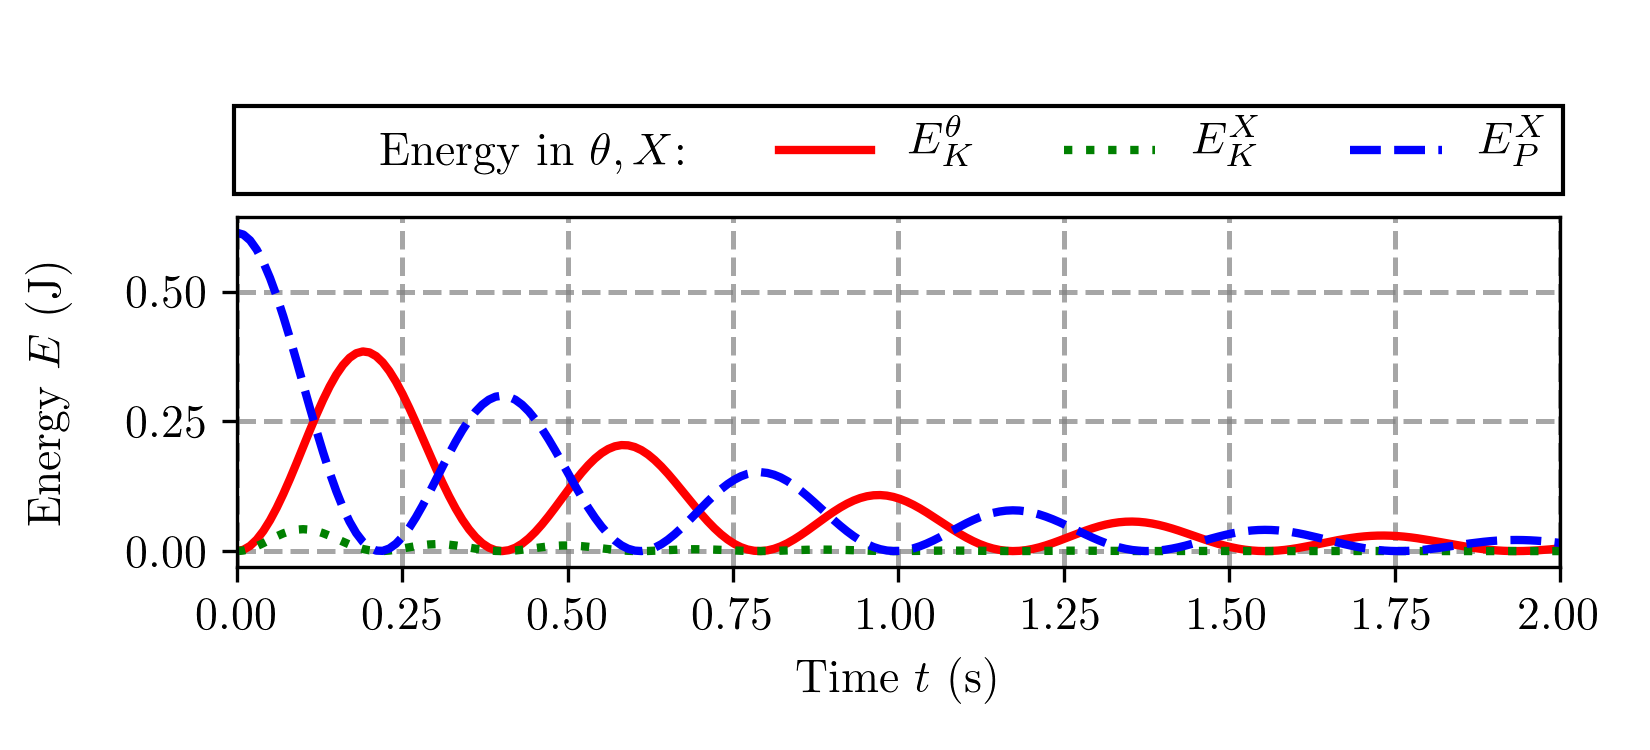
\includegraphics[trim= 0.0cm 0.8cm 0.0cm 0.0cm,width=1.0\columnwidth]{pics/plots/energy_damp.png}
		\caption{Simulated time plot of energy components: kinetic energy of the motor ($E_K^\theta$), payload ($E_K^X$) and potential energy of the latter ($E_P^X$)} 
 		\label{fig:energies_simulation}
		\vspace*{-2mm} 
\end{figure}


It follows from the simulation results that, unless energy dissipation is excessively large, one should be able to observe periodical motion of the system in the phase plane of actuator coordinates $\{\theta, \dot{\theta}\}$ and payload coordinates $\{X,\dot{X}\}$. Moreover, the phase trajectory in the motor space should theoretically lie in all four quadrants of the phase plane, while the payload's phase trajectory must be fully contained on the right hand side of the phase plane (since solution of \eqref{eq.mod:geom_const} with respect to $X$ is always positive) and pass through the origin $X = 0 , \dot{X} = 0$. Simulated phase plots are shown in Fig. \ref{fig:phase_plots_simulation}.

\begin{figure}
		\centering
		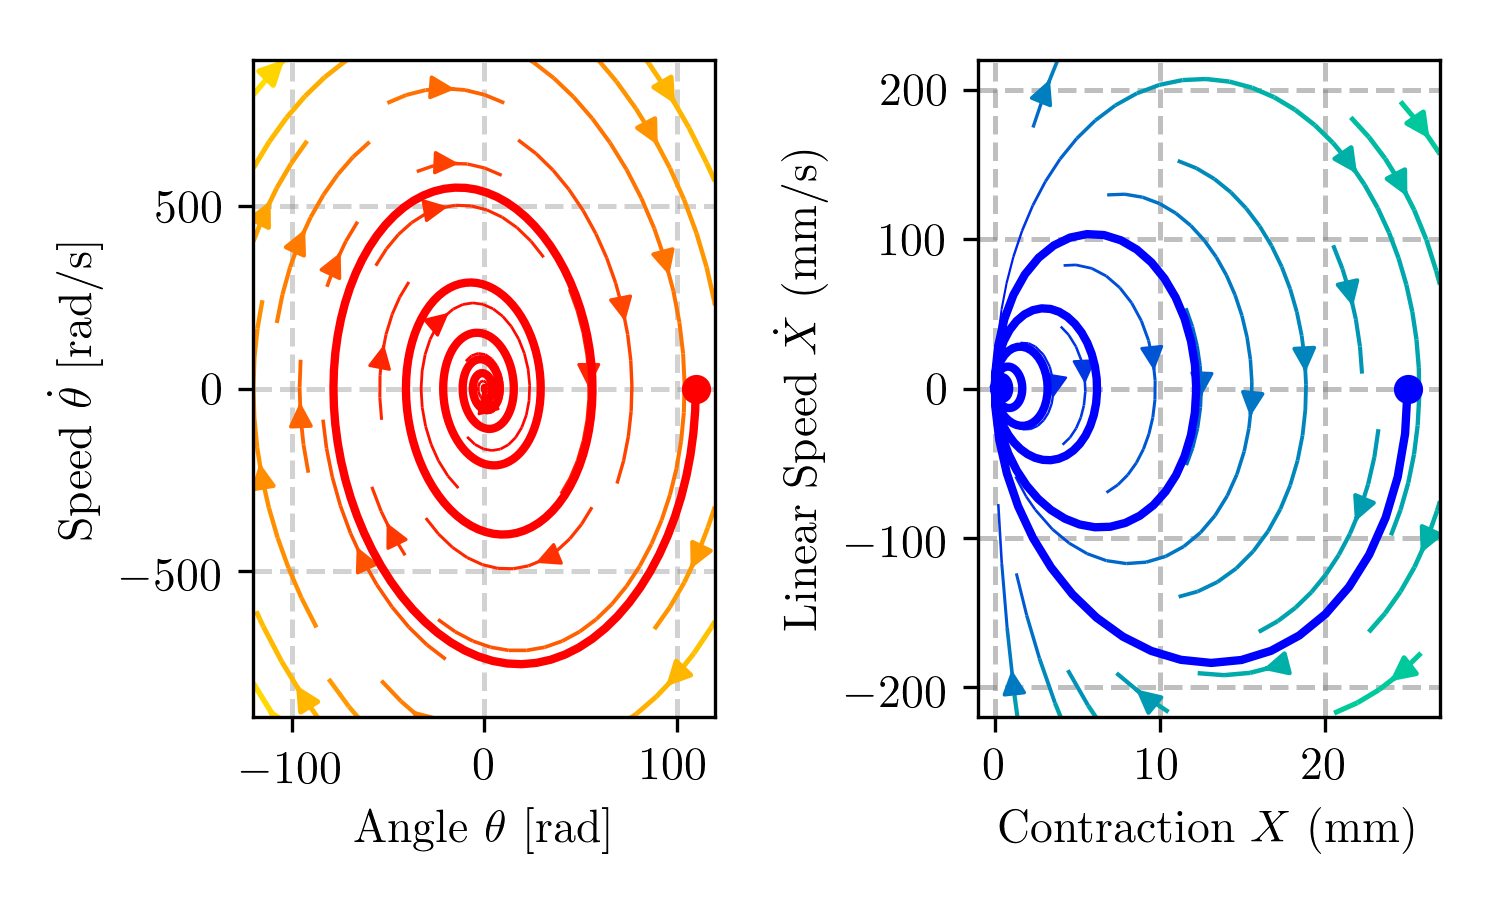
\includegraphics[trim= 0.0cm 0.8cm 0.0cm 0.0cm,width=1.0\columnwidth]{pics/plots/phase_space_model.png}
		\caption{Phase plots of damped oscillations in a TSA system in the motor (left) and payload (right) coordinates. Vector fields indicate the direction of motion in various points of the phase plot}
 		\label{fig:phase_plots_simulation}
		\vspace*{-2mm} 
\end{figure}

As the next step, we have decided to repeat the simulations whose results are presented in Fig. \ref{fig:energies_simulation} and \ref{fig:phase_plots_simulation} on a practical setup, and the experimental evaluation is described in the next section. 





\section{Energy, Phase Trajectories, and Periodic Orbits in TSA}
\label{orbits}
\subsection{Experimental Setup}
In order to investigate oscillations in twisted string actuators, we have manufactured the testbed shown in Fig.
\ref{fig:ex_setup}. It is comprised of a EC motor (Maxon EC-4pole 22 120W, 18V) equipped with a quadrature optical incremental encoder (1024 CPT), a linear encoder with the resolution of 18 $\mu$m (Avago H9740-1 360 LPI) 
to measure the actual string contraction and a digital controller (32 bit Arm Cortex-M7 216 MHz core-based) 
connected to the motor driver (ESCON 70/10). We have installed a pair of 0.75-mm Dyneema strings in the TSA with the length of 170 mm, just like the ones used in simulation. 

	\begin{figure}
		\centering
		\vspace*{-1mm} 
		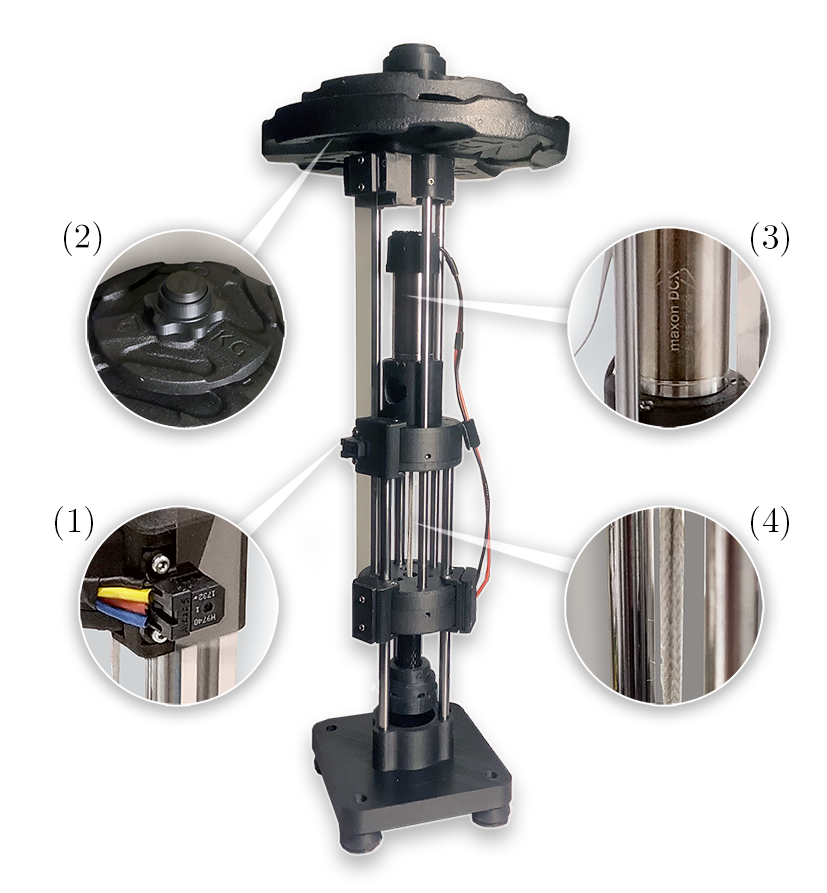
\includegraphics[trim= 0.0cm 0.5cm 0.0cm 0.0cm, width=0.8\columnwidth]{pics/linear_setup.png}
		\caption{Photo of the experimental setup:  1) linear encoder, 2) static payload, 3) EC motor with angular incremental encoder, 4) twisted strings  }
		\label{fig:ex_setup}
		\vspace*{-4mm} 
	\end{figure}

The setup operates as follows. The motor twists the strings, causing their contraction. The strings pull up the bottom mount which moves along three vertical sliders (fixed between the base and the motor mount) and has a optical strip attached to it. Rigidly fixed to the moving mount are three more thin metal rods that support the top platform with a payload. The motion of the optical strip is registered by a stationary optical encoder located at the motor mount.

\subsection{Energy and Phase Trajectories}
After we confirmed the presence of oscillations in a practical setup similar to those suggested by the simulations, our first aim was to try recreate the oscillatory energy behavior presented in Fig. \ref{fig:energies_simulation}. The corresponding experimental plot of major energy components in TSA is given in Fig. \ref{fig:energies_exp}. One can note the similarities between the simulated and experimental energy curves, with the main difference being a slightly lopsided shape of the actuator kinetic energy $E_K^\theta$. This is most likely caused by some effects at play in a practical setup which are not reflected by the simplified energy model, namely, dry friction and unilateral string stiffness (jamming) described in our previous work \cite{nedelchev2020accurate}. However, the general nature of the oscillations, as well as their frequency, was predicted by the simulated results fairly well.
\begin{figure}
		\centering
		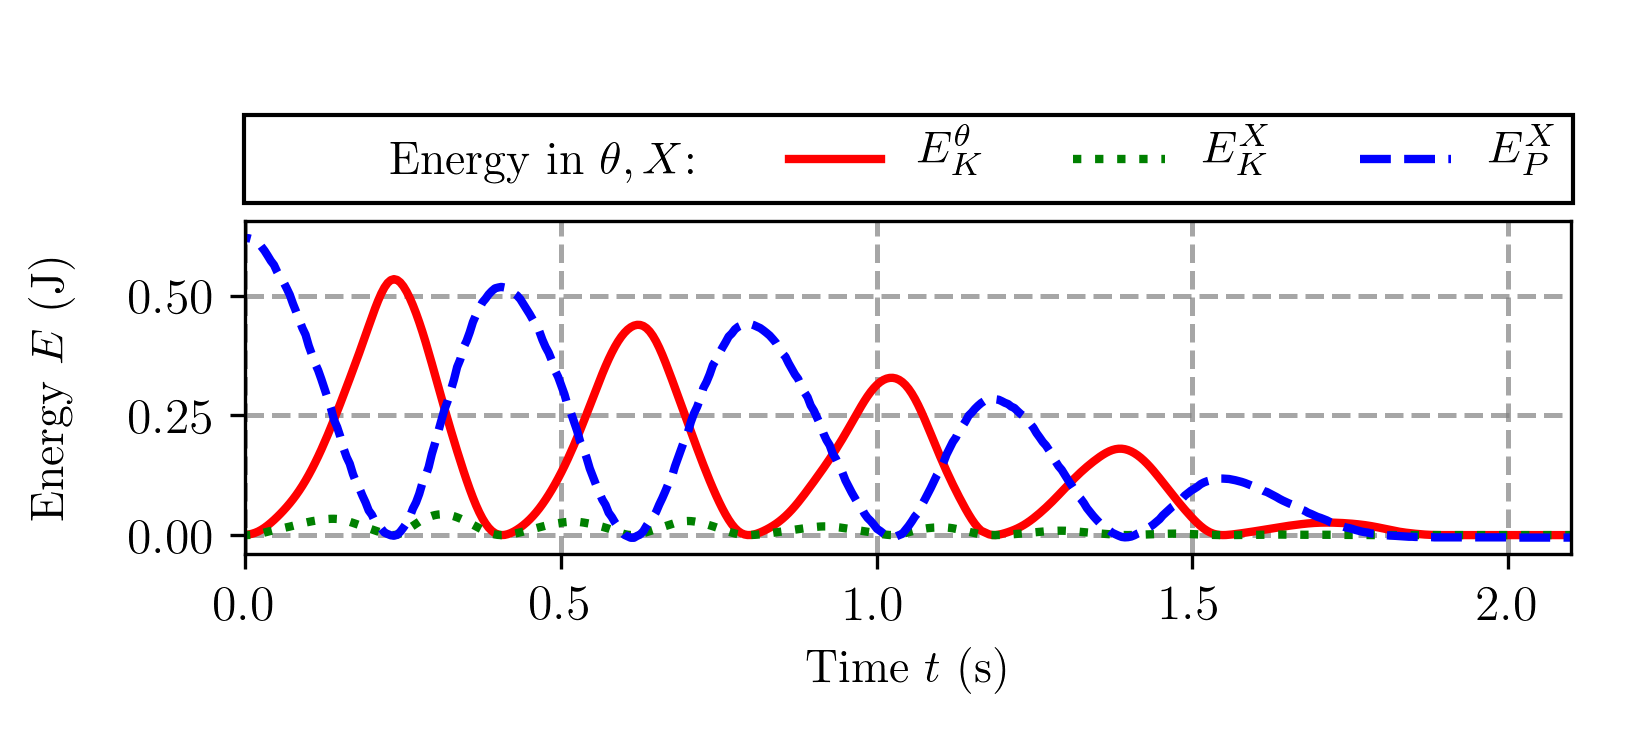
\includegraphics[trim= 0.0cm 1.0cm 0.0cm 0.0cm,width=1.0\columnwidth]{pics/plots/exp_energy_damp.png}
		\caption{Experimental time plots of energy components in a TSA during free oscillations with 90\% of friction compensated for by controller}
 		\label{fig:energies_exp}
		\vspace*{-2mm} 
\end{figure}

Corresponding phase plots in actuator and payload coordinates are presented in Fig. \ref{fig:phase_plots_exp}. Here, the shape difference between simulated and experimental phase trajectories are more apparent, which calls for a deeper analysis if one desires to predict the curves with higher accuracy. However, in this preliminary research we were mainly interested in whether we would be able to predict the peak values of positions and velocities (and the corresponding energy levels) with enough accuracy, and the simplified energy model allows to achieve this. 

\begin{figure}
		\centering
		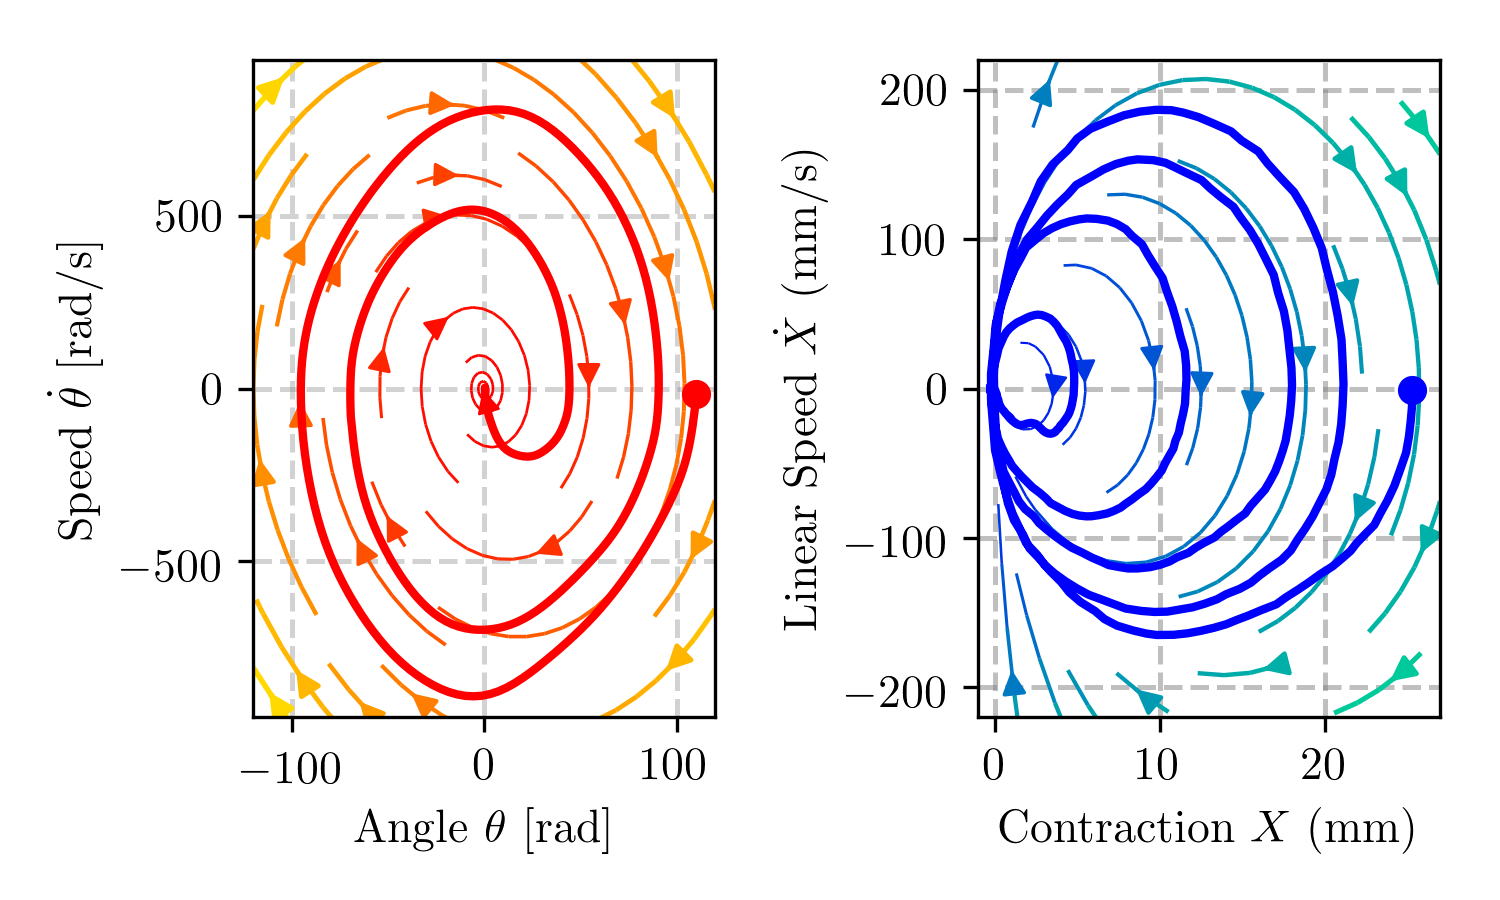
\includegraphics[trim= 0.0cm 1.0cm 0.0cm 0.0cm,width=1.0\columnwidth]{pics/plots/phase_space_experiment.png}
		\vspace*{-2mm} 
		\caption{Experimental phase plots of free oscillations, with the vector fields plotted with help of the proposed model}
 		\label{fig:phase_plots_exp}
\end{figure}

\subsection{Friction Compensation}
Once one has a satisfactory model of free oscillatory response in a twisted string actuator that is confirmed by experiments, one research question that can be asked is how can we use this knowledge to design an energy-efficient controller for TSAs. Since the main causes of power dissipation in the system are the frictional forces, their cancellation (or at least compensation for) would naturally prolong free oscillatory response in the actuator. Thus, we have designed a feedforward control system which would introduce the torque $u = \hat{b}\dot{\theta}$, with a positive term $\hat{b}$ representing our guess of viscous friction coefficient. 

A time plot of three curves, corresponding to damped oscillatory response of TSA for 3 different values of $\hat{b}$ are shown in Fig. \ref{fig:friction_cancellation}. One can note how increased friction compensation leads to prolonged   oscillations, as expected. Thus, if one can fully compensate for friction (e.g. with feedforward/feedback linearization) in a TSA system, it is possible to induce undamped oscillatory response in it with the `natural' frequency. Just like in any undamped system, total energy will remain constant during free oscillations, with kinetic energy of the actuator converted into kinetic and potential energy of the payload, and vice versa. The reverse is also true - if one preserves constant energy levels within a TSA-based system by means of control, they can induce undamped oscillations with minimal control effort, which can be leveraged, for example, when designing a legged robot. 

Energy preservation in TSA is studied in detail in the following section.
\begin{figure}
		\centering
		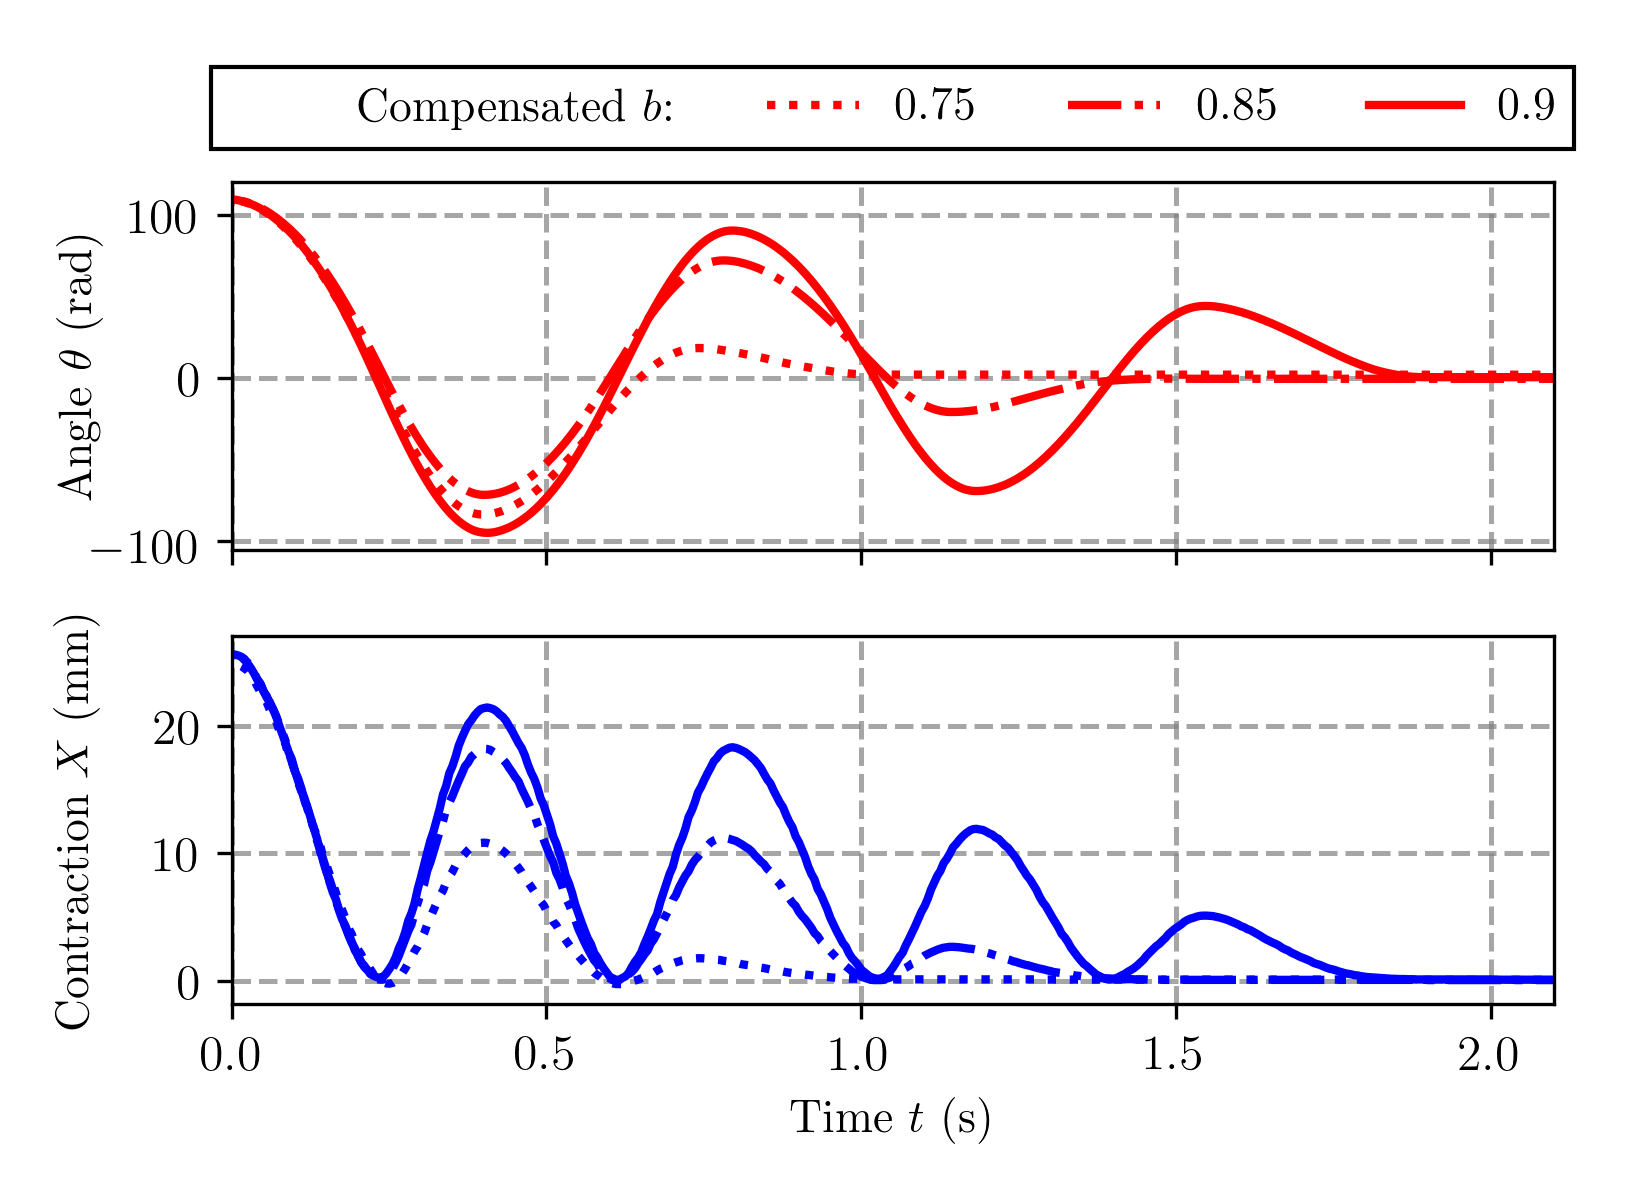
\includegraphics[trim= 0.0cm 1.0cm 0.0cm 0.0cm,width=1.0\columnwidth]{pics/plots/exp_var_damp.png}
		\caption{Time plots of motor angle (top) and payload (bottom) for various levels of friction compensation}
 		\label{fig:friction_cancellation}
		\vspace*{-2mm} 
\end{figure}



\section{Energy Preserving Control over TSA}
\label{control}
As discussed above, one can induce periodic undamped oscillations within TSAs by conserving mechanical energy of the system. This can be achieved by a proper selection of control algorithm, and this approach is commonly known in literature as energy preserving control (EPC). The following provides a brief introduction into the EPC and discusses design and implementation of this control strategy to twisted string actuators.

The concept of energy-preserving control has been originally proposed by Wiklund et al. who demonstrated an approach to solve the swing-up problem of inverted pendulum with this control strategy \cite{wiklund1993new}. The EPC technique was later applied to other underactuated systems (Furuta pendulum, acrobot, three-link gymnast robot, cart-pole) in the works of Iwashiro and Spong, with the studies outlining regulation methods to reach desired energy levels even in the presence of actuator constraints \cite{iwashiro1996energy,spong1996energy}.
Fantoni et al. have later demonstrated how, using the passivity properties of the internal energy of a pendubot system, one can bring the state either arbitrarily close to the top position or to some homoclinic orbit  \cite{fantoni2000energy}. %Research into energy-based control for the underactuated systems is still going on. % This is how real-time energy control of the cart-pole was presented in the article \cite{kennedy2019real}. This controller used a novel barrier function to make the swing-up method. This feature allows using the energy-based controller for real-time implementation.
%The sequence of papers by Maalouf and colleagues  \cite{maalouf2017energy,maalouf2020biomimetic} demonstrated the compatibility of energy-based control for humanoid robots in push recovery during quiet standing scenario. Case-study demonstrated that energy-based control is more efficient in terms of cumulative work than PID control and controlled Lagrangian approach. Additionally to energy efficiency, authors highlighted that energy-based control performance required in some setups the same (inverted pendulum on a cart) or up to 3 times lower-order (inverted pendulum) of peak control torque on actuator comparing with PID and controlled Lagrangian. This property of energy-based control could be used in low-power motor systems.
In addition, the EPC was successfully applied in robot control tasks. For instance, Asano et al. have used this technique to control a bipedal walking robot and discovered that the application of energy constraints has significantly simplified generation of movement patterns \cite{asano2004novel}.

\subsection{Fundamentals of Energy-Preserving Control}

One of the most powerful features of the energy preserving control method is that it becomes much simpler to design a regulator for a particular dynamical system. One starts the EPC design process by driving a single energy equation of the system $E(q)$, where $q$ is a scalar position. In order to reach some desired position $q_d$, one therefore needs to reach constant desired energy level $E_d = E(q_d)$. Then, defining the energy error with
\begin{equation*}
    \tilde{E} = E_d - E(q)
\end{equation*}
and choosing control law as
\begin{equation}\label{eq.con:epc}
    u = k\tilde{E}\dot{q}
\end{equation}
results in energy error converging to zero, which will eventually drive system energy to desired level $E_d$. This may be shown by analyzing the Lyapunov candidate 
\begin{equation}\label{eq:v_dot}
    V = \frac{1}{2}\tilde{E}^2
\end{equation}
whose derivative can be found as follows:
\begin{equation}\label{eq:v_dot}
    \dot{V} = \tilde{E}\dot{\tilde{E}} = \tilde{E} ( \dot{E}_d - \dot{q} u) = -\tilde{E} \dot{q}^T u= -k\tilde{E}^2\dot{q}^2
\end{equation}
which is strictly negative along all system trajectories, provided that $\dot{q}\neq0$. For more details on stability analysis of this control scheme the reader is kindly referred to the works \cite{iwashiro1996energy,spong1996energy}.

Now, let us move onto implementation of energy preserving control in the linear TSA joint studied in the previous section.
 
\subsection{Experiment with a Linear TSA}

We have conducted an experiment whose main goal was to induce TSAs load oscillation with amplitude of $X_d = 20$ mm starting from a fully untwisted configuration. the mass was setted to be $\hat{m} = 2$ kg which corresponds to the energy level of $E = 0.39$ J. In addition, maximal motor torque was set to be 6 mNm. 

In order to regulate to the desired energy level we have implemented control law \eqref{eq.con:epc}, with actual energy provided by equation \eqref{eq.mod:total_energy} except for the dissipative term $E_D$: 
\begin{equation}\label{eq.con:total_energy}
    E = \frac{1}{2} \hat{I}\dot{\theta}^2 + \frac{1}{2}\hat{m} \dot{X}^2 + \hat{m}gX
\end{equation}
where $\hat{I}, \hat{m}$ denote our estimates of the motor inertia and payload mass, respectively. The value of motor inertia was identified to be $\hat{I}=9.7$ gcm$^2$. 
Load position $X$ was measured directly while $\dot{\theta},\dot{X}$ was estimated with backward difference with data sampling frequency of 3 kHz. No other computations or measurements were necessary for energy calculations.

Time plots of resulting payload motion and motor torque are presented in Figure \ref{fig:time_plots_X_torque_epc}. One can note that it takes the controller about 2.5 periods in as many seconds to reach desired contraction levels, while the motor torque remains bounded. Motor controller had a hardware cutoff at 6 mNm torque, which is shown by a horizontal dashed line in  Fig. \ref{fig:time_plots_X_torque_epc} (bottom), while the intermittent peaks exceeding these values are the result of noise in electrical current measurements that were used to compute motor torque.
For the sake of comparison, if one simply commands the motor to twist the strings and drive the payload to the desired contraction level with the same torque constraint of 6 mNm, the load gets after travelling approximately 3 mm, as shown by the curve labeled `PD control' in Fig. \ref{fig:time_plots_X_torque_epc} (top). 

\begin{figure}
		\centering
		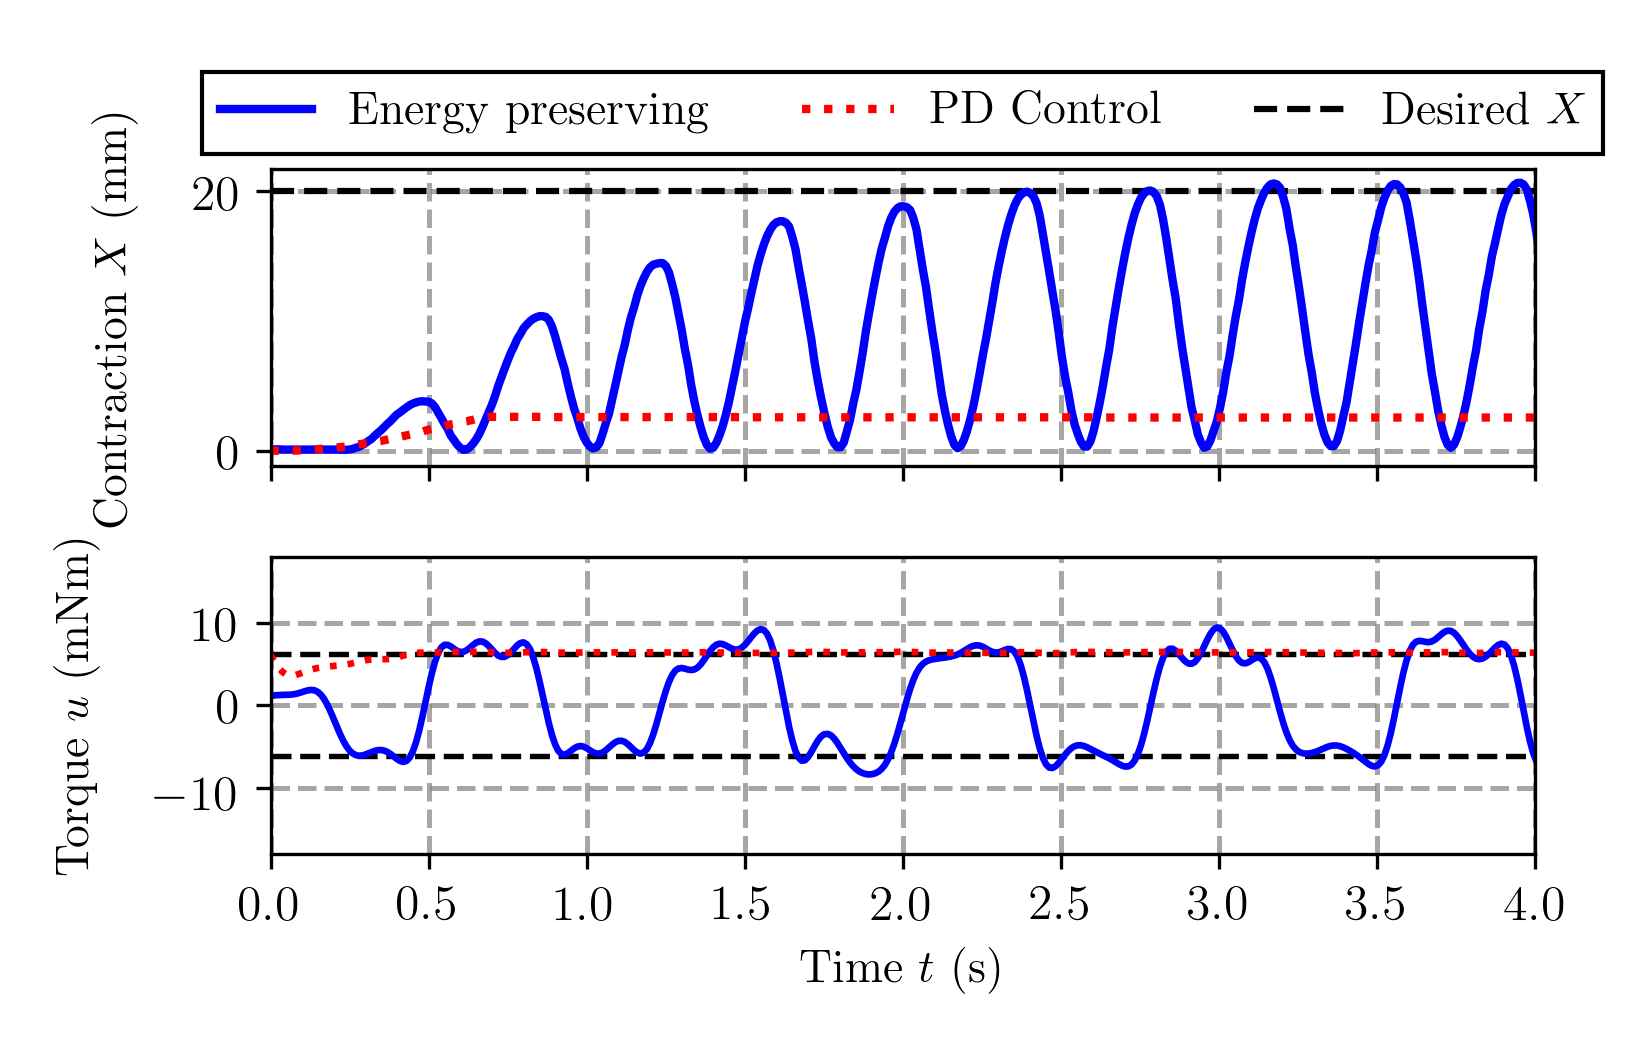
\includegraphics[trim= 0.0cm 0.8cm 0.0cm 0.0cm,width=1.0\columnwidth]{pics/plots/control_comparison.png}
		\caption{Experimental time plots of payload position (top) and motor torque (bottom) in a TSA with energy-preserving control and torque constraints}
 		\label{fig:time_plots_X_torque_epc}
		\vspace*{-2mm} 
\end{figure}

Once the desired energy level has been reached, the controller conserves it throughout the experiment, as shown in Fig. \ref{fig:energy_levels_EPC}. The corresponding phase plots in the actuator and payload space are shown in Fig. \ref{fig:phase_plot_EPC}. One can note with the help of overlaid vector fields (computed with the proposed mathematical model) that oscillations starting from the origin diverge toward the final limit cycle, while those that start outside converge to it, which suggests stable controller behavior. The same observation holds for both motor and payload responses.
\begin{figure}
		\centering
		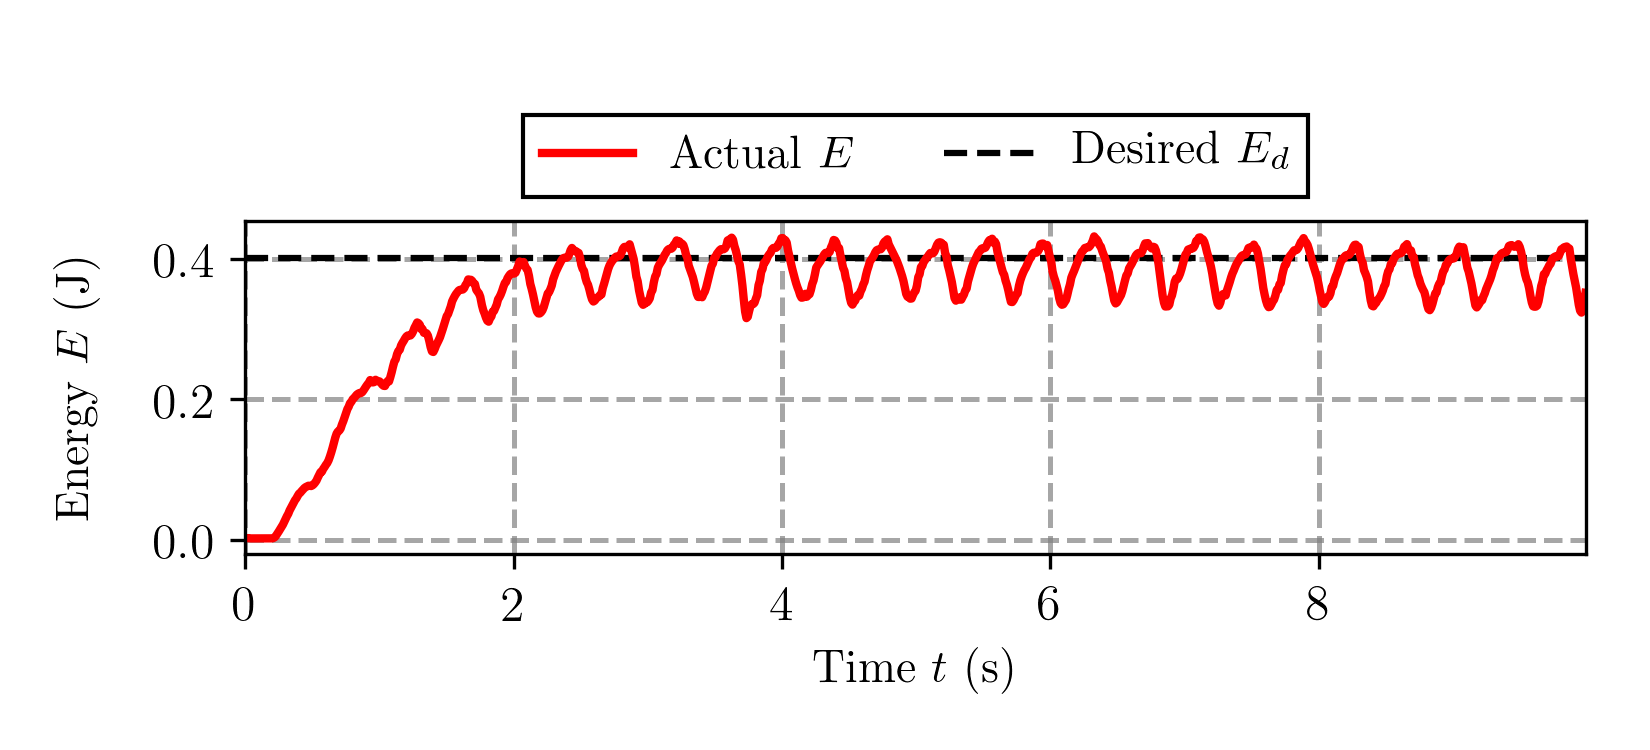
\includegraphics[trim= 0.0cm 1.0cm 0.0cm 0.0cm,width=1.0\columnwidth]{pics/plots/energy_convergence.png}
		\caption{Desired and actual energy levels in TSA under energy preserving control}
 		\label{fig:energy_levels_EPC}
		\vspace*{-2mm} 
\end{figure}

\begin{figure}
		\centering
		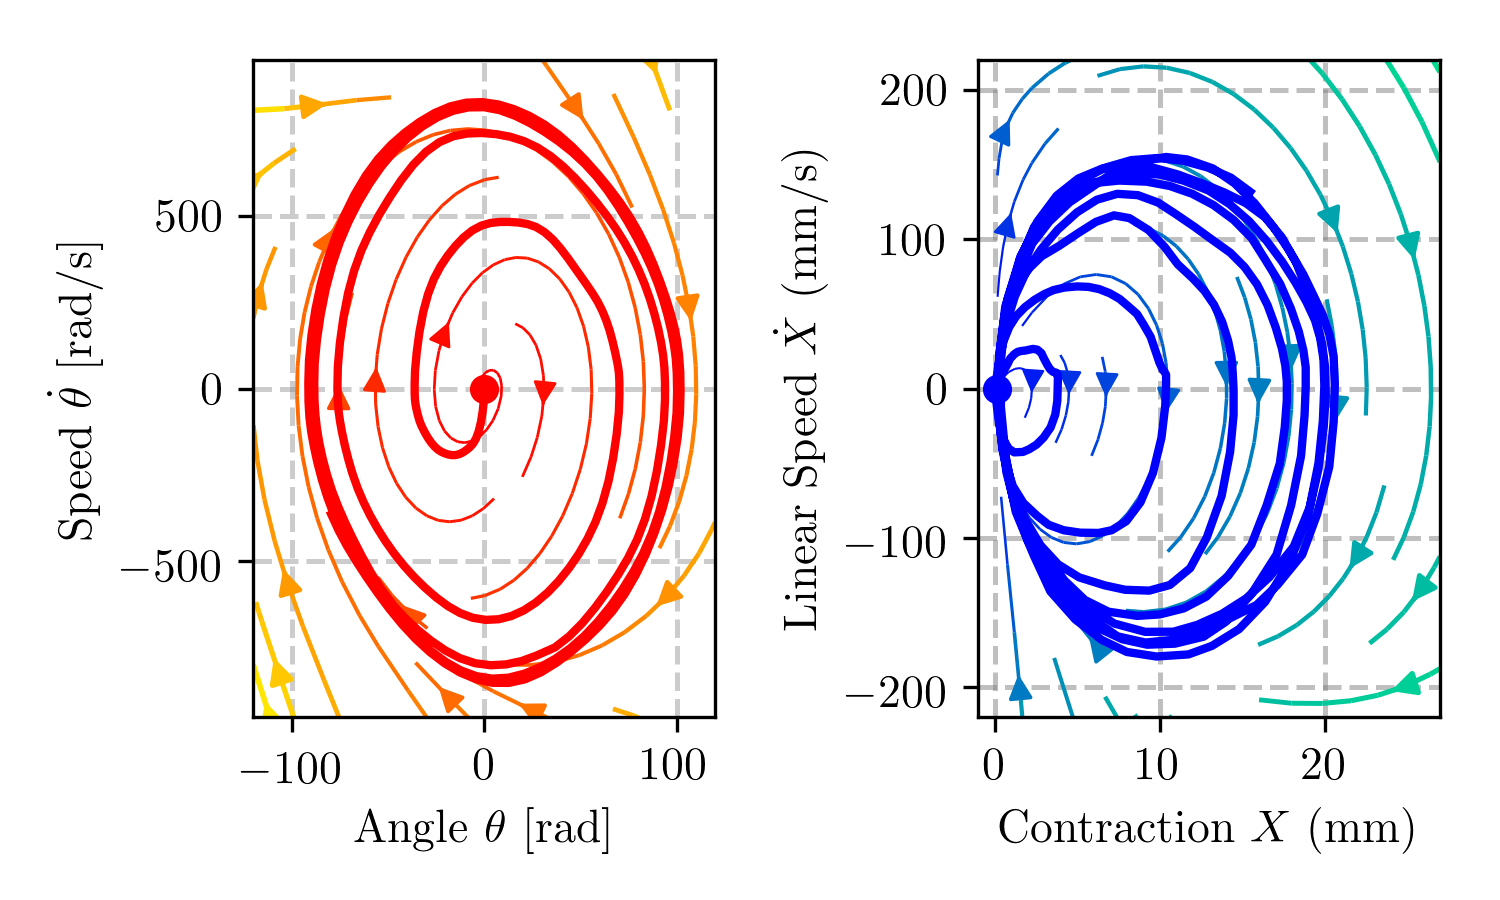
\includegraphics[trim= 0.0cm 0.8cm 0.0cm 0.0cm,width=1.0\columnwidth]{pics/plots/phase_space_control.png}
		\caption{Phase portraits of TSA in actuator (left) and payload (right) space with energy preserving control. Vector fields are generated with proposed mathematical model}
 		\label{fig:phase_plot_EPC}
		\vspace*{-2mm} 
\end{figure}

These experiments confirm that energy preserving control can indeed be successfully implemented in twisted string actuators to generate undamped oscillatory response with nearly-constant energy levels, as was suggested by our initial hypothesis. Design of controllers of this type is fairly simple and straightforward, and therefore these results seem very encouraging. 



\section{Conclusion}
\label{conclusion}

In this paper, we investigated free oscillatory response of linear twisted string actuators. We have outlined a mathematical model based on energy observations and TSA dynamics that could predict the oscillations with satisfactory accuracy and described energy conversion within TSA. 

One important consequence of understanding the nature of oscillatory responses in twisted string actuators is the ability to design TSA-based robotic systems that could efficiently leverage the advantages of this oscillatory process for the purposes of control. As one example, with appropriate controller selection one can deliberately induce undamped oscillatory response in TSA by preserving mechanical energy within a system at a desired level. We have implemented one such technique (energy-preserving control) and validated it in a series of hardware experiments. The tests have demonstrated that it was possible to generate undamped oscillatory response in a TSA with a payload of 2 kg while exerting a maximum of 6 mNm torque. This suggests that energy preserving control can be used in combination with TSA to ensure power-efficient locomotion, and this control strategy can also be used in applications that pose high requirements to power efficiency and require periodic movements of a certain magnitude.

In the simplest TSA module like the one studied in this paper, we can only control the magnitude of the oscillations and not their frequency. However, if one introduces an element with variable stiffness, it should become possible to control both frequency and magnitude, thus supporting a more diverse range of periodic motions. This can be beneficial for applications like legged robots that may require different gaits depending on a situation, or for robots whose dynamical parameters can vary significantly during periodic movements.

In the nearest future, we are planning to investigate oscillations and extend energy preserving control to rotational TSA-based systems. In addition, we are planning to design a 2-DOF robotic legged that employs TSAs, induce oscillatory response and investigate the effects of contact with environment (hybrid dynamics) on system behavior. When developing TSA-based robotic limbs, one can design their movement trajectories in such a way that they are as close to oscillations as possible. Once designed, the controller will stabilize the resulting orbits.
    %\section*{Acknowledgment}
    


    \addtolength{\textheight}{-12cm}   % This command serves to balance the column lengths
    % on the last page of the document manually. It shortens
    % the textheight of the last page by a suitable amount.
    % This command does not take effect until the next page
    % so it should come on the page before the last. Make
    % sure that you do not shorten the textheight too much.


	\bibliographystyle{IEEEtran}
	%%use following if all content of bibtex file should be shown
%	\nocite{*}
	\bibliography{ref}

\end{document}